\section{Experiment}

\subsection{Configuration}
\begin{frame}
    \frametitle{Configuration}
    \begin{itemize}
    	\item Four versions
		    \begin{itemize}
				\item \textit{LOOPDP}: optimized looping code with padding
					to mitigate set-associativity problem.
				\item \textit{CO}: unoptimized CORDAC.
				\item \textit{CO\_Opt}: optimized CORDAC + copy-optimization.
				\item \textit{COZ}: \textit{CO\_Opt} + \textit{ZM\_RM} 
					layout for data storage.
			\end{itemize}
		\item Base-case size of $64 \times 64$ for parenthesis, gap and protein 
			folding and $128 \times 128$ for FW-APSP.
	\end{itemize}
\end{frame}

\subsection{Platforms}
\begin{frame}
    \frametitle{Platforms}
    \begin{figure}
		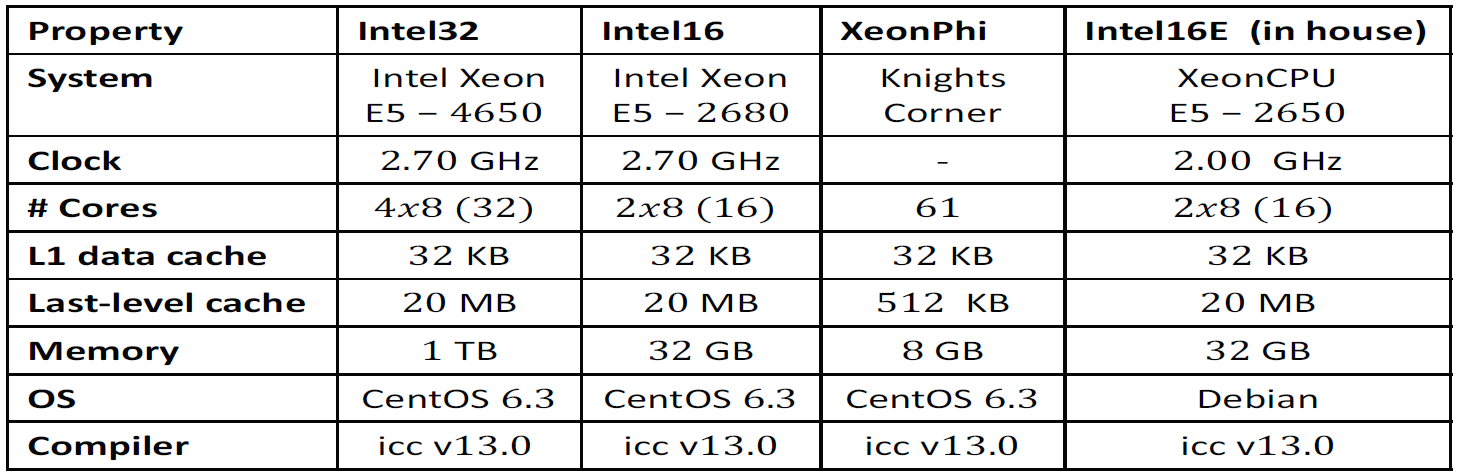
\includegraphics[scale=0.3]{figure/fig-platforms.png}
	\end{figure}
\end{frame}

\subsection{Shared-Memory Machine}
\begin{frame}
    \frametitle{Performance on Shared-Memory Machine}
    \begin{itemize}
    	\item For parenthesization problem, hybrid CPU + 
    		Xeon Phi version runs $395\times$ for $n = 32768$.
    	\item Explicit vectorization contributed up to $5\times$ speedup
    		over auto-vectorized code.
    	\item CORDAC algorithms consume $4$ -- $30\times$ less energy.
    \end{itemize}
\end{frame}

\begin{frame}
    \begin{figure}
		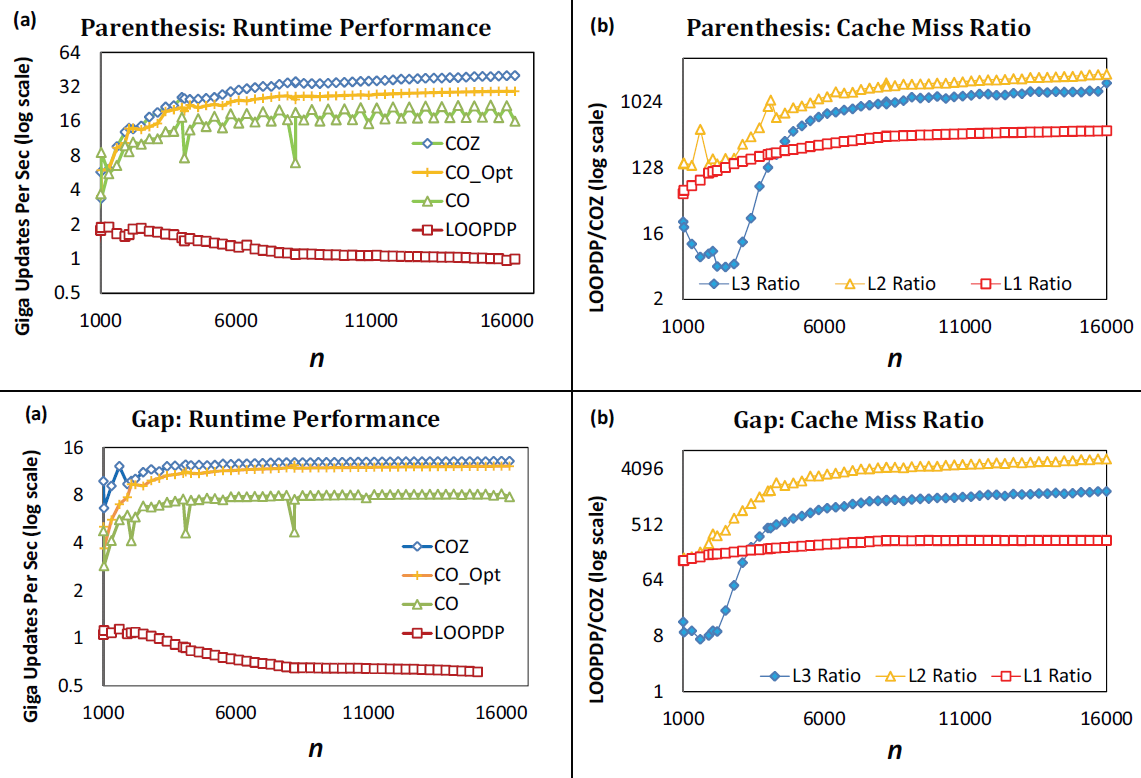
\includegraphics[scale=0.3]{figure/fig-shared-machine-1.png}
	\end{figure}
	\footnote{Performance on Intel 16: Intel Xeon E5-2680}
\end{frame}

\begin{frame}
    \begin{figure}
		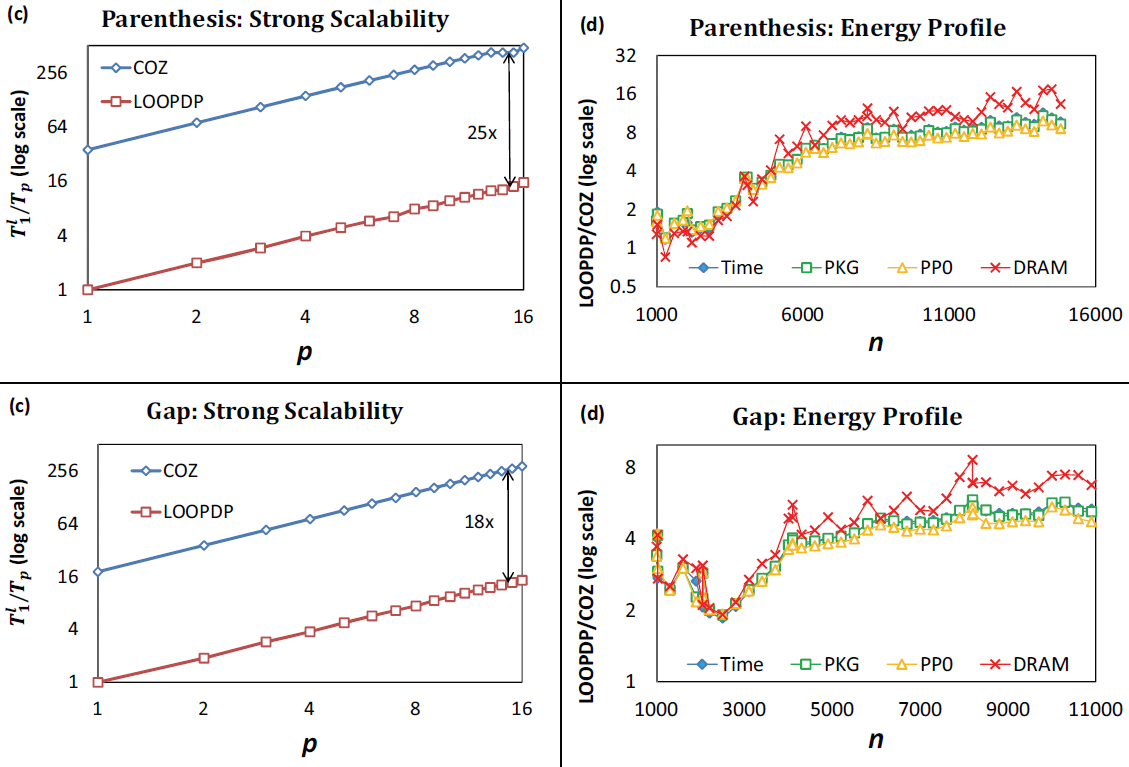
\includegraphics[scale=0.3]{figure/fig-shared-machine-2.png}
	\end{figure}
	\footnote{Performance on Intel 16: Intel Xeon E5-2680}
\end{frame}
